\documentclass[11pt,a4paper]{article}
\usepackage{graphicx,latexsym,isabelle,isabellesym,latexsym,pdfsetup}

\urlstyle{tt}
\pagestyle{myheadings}

\addtolength{\hoffset}{-1,5cm}
\addtolength{\textwidth}{4cm}
\addtolength{\voffset}{-2cm}
\addtolength{\textheight}{4cm}

%remove spaces from the isabelle environment (trivlist makes them too large)
\renewenvironment{isabelle}
{\begin{isabellebody}}
{\end{isabellebody}}

\newcommand{\nJava}{\it NanoJava}

%remove clutter from the toc
\setcounter{secnumdepth}{3}
\setcounter{tocdepth}{2}

\begin{document}

\title{\nJava}
\author{David von Oheimb \\ Tobias Nipkow}
\maketitle

\begin{abstract}\noindent
  These theories define {\nJava}, a very small fragment of the programming 
  language Java (with essentially just classes) derived from the one given 
  in \cite{NipkowOP00}.
  For {\nJava}, an operational semantics is given as well as a Hoare logic,
  which is proved both sound and (relatively) complete. 
  The Hoare logic supports side-effecting expressions and
  implements a new approach for handling auxiliary variables.
  A more complex Hoare logic covering a much larger subset of Java is described
  in \cite{DvO-CPE01}.\\
See also the homepage of project Bali at \url{http://isabelle.in.tum.de/Bali/}
and the conference version of this document \cite{NanoJava}.
\end{abstract}

\tableofcontents
\parindent 0pt \parskip 0.5ex

\begin{center}
  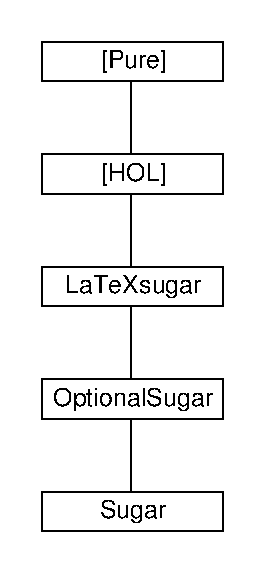
\includegraphics[scale=0.7]{session_graph}  
\end{center}

\newpage
%
\begin{isabellebody}%
\def\isabellecontext{a{\isadigit{6}}}%
\isamarkupfalse%
%
\isamarkupsubsection{Optimising Compiler Verification%
}
\isamarkuptrue%
%
\begin{isamarkuptext}%
Section 3.3 of the Isabelle tutorial describes an expression compiler for a stack machine. In this exercise we will build and verify an optimising expression compiler for a register machine.%
\end{isamarkuptext}%
\isamarkuptrue%
%
\begin{isamarkuptext}%
\subsubsection*{The Source Language: Expressions}%
\end{isamarkuptext}%
\isamarkuptrue%
%
\begin{isamarkuptext}%
The arithmetic expressions we will work with consist of variables, constants, and an arbitrary binary operator \isa{oper}.%
\end{isamarkuptext}%
\isamarkuptrue%
\isacommand{consts}\ oper\ {\isacharcolon}{\isacharcolon}\ {\isachardoublequote}nat\ {\isasymRightarrow}\ nat\ {\isasymRightarrow}\ nat{\isachardoublequote}\isanewline
\isanewline
\isamarkupfalse%
\isacommand{types}\ var\ {\isacharequal}\ string\isanewline
\isanewline
\isamarkupfalse%
\isacommand{datatype}\ exp\ {\isacharequal}\ \isanewline
\ \ \ \ Const\ nat\ \isanewline
\ \ {\isacharbar}\ Var\ var\isanewline
\ \ {\isacharbar}\ Op\ exp\ exp\isamarkupfalse%
%
\begin{isamarkuptext}%
The state in which an expression is evaluated is modelled by an {\em environment} function that maps variables to constants.%
\end{isamarkuptext}%
\isamarkuptrue%
\isacommand{types}\ env\ {\isacharequal}\ {\isachardoublequote}var\ {\isasymRightarrow}\ nat{\isachardoublequote}\isamarkupfalse%
%
\begin{isamarkuptext}%
Define a function \isa{value} that evaluates an expression in a given environment.%
\end{isamarkuptext}%
\isamarkuptrue%
\isacommand{consts}\ value\ {\isacharcolon}{\isacharcolon}\ {\isachardoublequote}exp\ {\isasymRightarrow}\ env\ {\isasymRightarrow}\ nat{\isachardoublequote}\isamarkupfalse%
%
\begin{isamarkuptext}%
\subsubsection*{The Register Machine}%
\end{isamarkuptext}%
\isamarkuptrue%
%
\begin{isamarkuptext}%
As the name suggests, a register machine uses a collection of registers to store intermediate results. There exists a special register, called the accumulator, that serves as an implicit argument to each instruction. The rest of the registers make up the register file, and can be randomly accessed using an index.%
\end{isamarkuptext}%
\isamarkuptrue%
\isacommand{types}\ regIndex\ {\isacharequal}\ nat\isanewline
\isanewline
\isamarkupfalse%
\isacommand{datatype}\ cell\ {\isacharequal}\ \isanewline
\ \ \ \ Acc\isanewline
\ \ {\isacharbar}\ Reg\ regIndex\isamarkupfalse%
%
\begin{isamarkuptext}%
The state of the register machine is denoted by a function that maps storage cells to constants.%
\end{isamarkuptext}%
\isamarkuptrue%
\isacommand{types}\ state\ {\isacharequal}\ {\isachardoublequote}cell\ {\isasymRightarrow}\ nat{\isachardoublequote}\isamarkupfalse%
%
\begin{isamarkuptext}%
The instruction set for the register machine is defined as follows:%
\end{isamarkuptext}%
\isamarkuptrue%
\isacommand{datatype}\ instr\ {\isacharequal}\ \isanewline
\ \ LI\ nat\ \ \ \ \ \ \ \ \isanewline
\ \ %
\isamarkupcmt{Load Immediate: loads a constant into the accumulator.%
}
\ \isanewline
{\isacharbar}\ LOAD\ regIndex\ \isanewline
\ \ %
\isamarkupcmt{Loads the contents of a register into the accumulator.%
}
\isanewline
{\isacharbar}\ STORE\ regIndex\ \isanewline
\ \ %
\isamarkupcmt{Saves the contents of the accumulator in a register.%
}
\ \isanewline
{\isacharbar}\ OPER\ regIndex\ \isanewline
\ \ %
\isamarkupcmt{Performs the binary operation \isa{oper}.%
}
\isanewline
\ \ \ \ %
\isamarkupcmt{The first argument is taken from a register.%
}
\isanewline
\ \ \ \ %
\isamarkupcmt{The second argument is taken from the accumulator.%
}
\ \isanewline
\ \ \ \ %
\isamarkupcmt{The result of the computation is stored in the accumulator.%
}
\isamarkupfalse%
%
\begin{isamarkuptext}%
A program is a list of such instructions. The result of running a program is a change of state of the register machine. Define a function \isa{exec} that models this.%
\end{isamarkuptext}%
\isamarkuptrue%
\isacommand{consts}\ exec\ {\isacharcolon}{\isacharcolon}\ {\isachardoublequote}state\ {\isasymRightarrow}\ instr\ list\ {\isasymRightarrow}\ state{\isachardoublequote}\isamarkupfalse%
%
\begin{isamarkuptext}%
\subsubsection*{Compilation}%
\end{isamarkuptext}%
\isamarkuptrue%
%
\begin{isamarkuptext}%
The task now is to translate an expression into a sequence of instructions that computes it. At the end of execution, the result should be stored in the accumulator.

Before execution, the values of each variable need to be stored somewhere in the register file. A {\it mapping} function maps variables to positions in the register file.%
\end{isamarkuptext}%
\isamarkuptrue%
\isacommand{types}\ map\ {\isacharequal}\ {\isachardoublequote}var\ {\isasymRightarrow}\ regIndex{\isachardoublequote}\isamarkupfalse%
%
\begin{isamarkuptext}%
Define a function \isa{cmp} that compiles an expression into a sequence of instructions. The evaluation should proceed in a bottom-up depth-first manner.

State and prove a theorem expressing the correctness of \isa{cmp}.

Hints:
\begin{itemize}
  \item The compilation function is dependent on the mapping function.
  \item The compilation function needs some way of storing intermediate results. It should be clever enough to reuse registers it no longer needs.
  \item It may be helpful to assume that at each recursive call, compilation is only allowed to use registers with indices greater than a given value to store intermediate results.
\end{itemize}%
\end{isamarkuptext}%
\isamarkuptrue%
%
\begin{isamarkuptext}%
\subsubsection*{Compiler Optimisation: Common Subexpressions}%
\end{isamarkuptext}%
\isamarkuptrue%
%
\begin{isamarkuptext}%
In the previous section, the compiler \isa{cmp} was allowed to evaluate a subexpression every time it occurred. In situations where arithmetic operations are costly, one may want to compute commonly occurring subexpressions only once.

For example, to compute \isa{{\isacharparenleft}a\ op\ b{\isacharparenright}\ op\ {\isacharparenleft}a\ op\ b{\isacharparenright}}, \isa{cmp} was allowed three calls to \isa{oper}, when only two were needed.

Develop an optimised compiler \isa{optCmp}, that evaluates every commonly occurring subexpression only once. Prove its correctness.%
\end{isamarkuptext}%
\isamarkuptrue%
\isamarkupfalse%
\end{isabellebody}%
%%% Local Variables:
%%% mode: latex
%%% TeX-master: "root"
%%% End:


%%% Local Variables:
%%% mode: latex
%%% TeX-master: "root"
%%% End:


\newpage
\nocite{*}
\bibliographystyle{abbrv}
\bibliography{root}

\end{document}
